\section{{\sys} 系统概览}
\label{sec:overview}

\definecolor{boxcolor}{HTML}{FFFFFF}
\definecolor{boxcolortwo}{HTML}{FFF6E6}

\newcommand{\fboxone}[1][1em]{%
  \tikz\filldraw[fill=boxcolor,draw=black] (0,0) rectangle (#1,#1);
}

\newcommand{\fboxtwo}[1][1em]{%
  \tikz\filldraw[fill=boxcolortwo,draw=black] (0,0) rectangle (#1,#1);
}

\begin{figure}[!t]
    \begin{minipage}{1\linewidth}
        \hspace{-1mm}
        \centering
        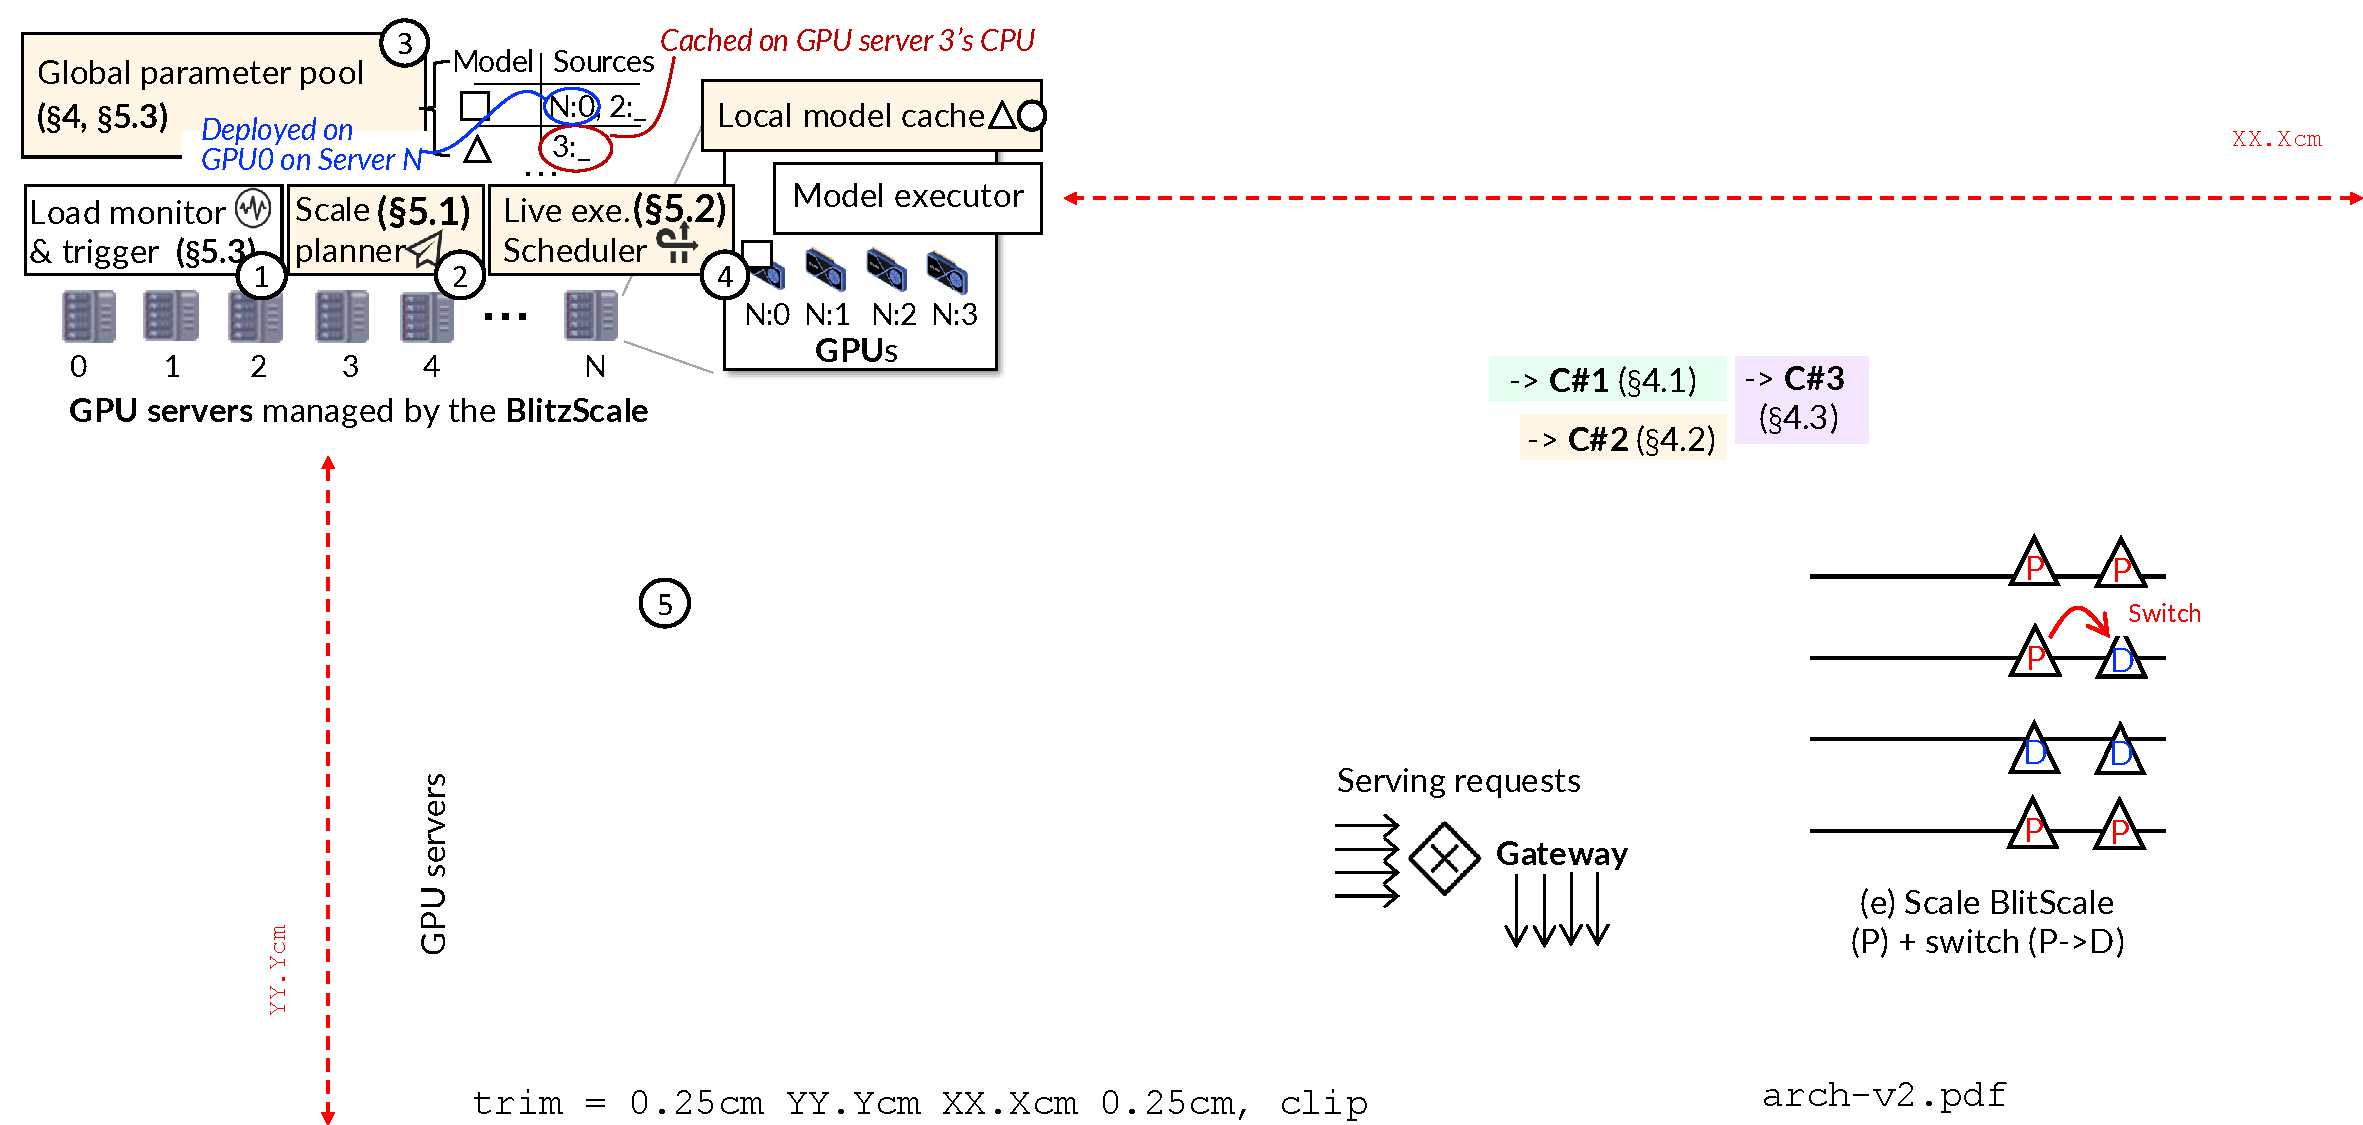
\includegraphics[width=.99\textwidth, trim=0.25cm 11.6cm 22.3cm 0.25cm, clip]{figs/arch-v2.pdf} \\[1pt]
    \end{minipage} \\[3pt]
    \begin{minipage}{1\linewidth}
        \caption{\small{\textit{
            {\sys} 的系统架构。
            由 {\sys} 新引入的模块用 {\fboxtwo} 标出。
        }}}
        \label{fig:arch}
    \end{minipage} \\[-10pt]
\end{figure}

\noindent
{\sys} 通过计算网络对模型进行扩缩，
即便主机缓存未命中，也能保持较快的扩缩速度。
为此，我们首先通过一个全局参数管理器来统一管理模型参数——
这些参数可能分散在服务实例背后的 GPU 上（针对已部署模型），
也可能位于主机 CPU 的缓存中。
该管理器维护模型与其参数来源之间的映射关系。
借助这一映射，
我们就能通过 RDMA 或 NVLink 这类高速互连，
迅速从相应来源读取参数。
除此之外，
我们还会把部分计算从过载实例卸载到那些仅完成部分参数加载的新实例上，
以实现在线扩缩容。

\stitle{系统架构与工作流程。\,}
{\fig{fig:arch}} 展示了系统架构。
与已有工作~\cite{DBLP:conf/usenix/Romero0YK21,DBLP:journals/corr/abs-2401-14351,DBLP:conf/osdi/SunHZXZL024} 类似，
我们有一个负载监控器（\ding{192}），
用于跟踪每个模型服务的负载情况，
并决定是否需要扩缩以及应扩出多少新实例（见 \textsection{\ref{sec:design-others}}）。
在每台机器上，
我们进一步采用现成的高性能 GPU kernel——FlashInfer~\cite{flashinfer}——来高效查询模型。
与现有系统相比，
{\sys} 的关键差异有两点。
第一，我们的扩缩规划器（\ding{193}）会结合全局参数管理器（\ding{194}）提供的信息，
生成一个扩缩计划，
用于指导如何通过计算网络高效地把参数加载到新扩出的实例上（见 \textsection{\ref{sec:design-plan}}）。
在图中的例子里，
新的实例既可以从主机 N 的 GPU0（记为 $(N,0)$）获取模型 {$\square$} 的参数，
也可以从主机 2 的 CPU 内存（记为 $(2,\_)$）获取。
第二，在扩缩期间，
我们的在线执行调度器（\ding{195}）会在实例之间重定向请求，
从而在参数尚未全部加载完成之前，就尽可能利用新实例的算力（见 \textsection{\ref{sec:design-pp}}）。

\begin{figure}[!t]
    \begin{minipage}{1\linewidth}
        \hspace{-1mm}
        \centering
        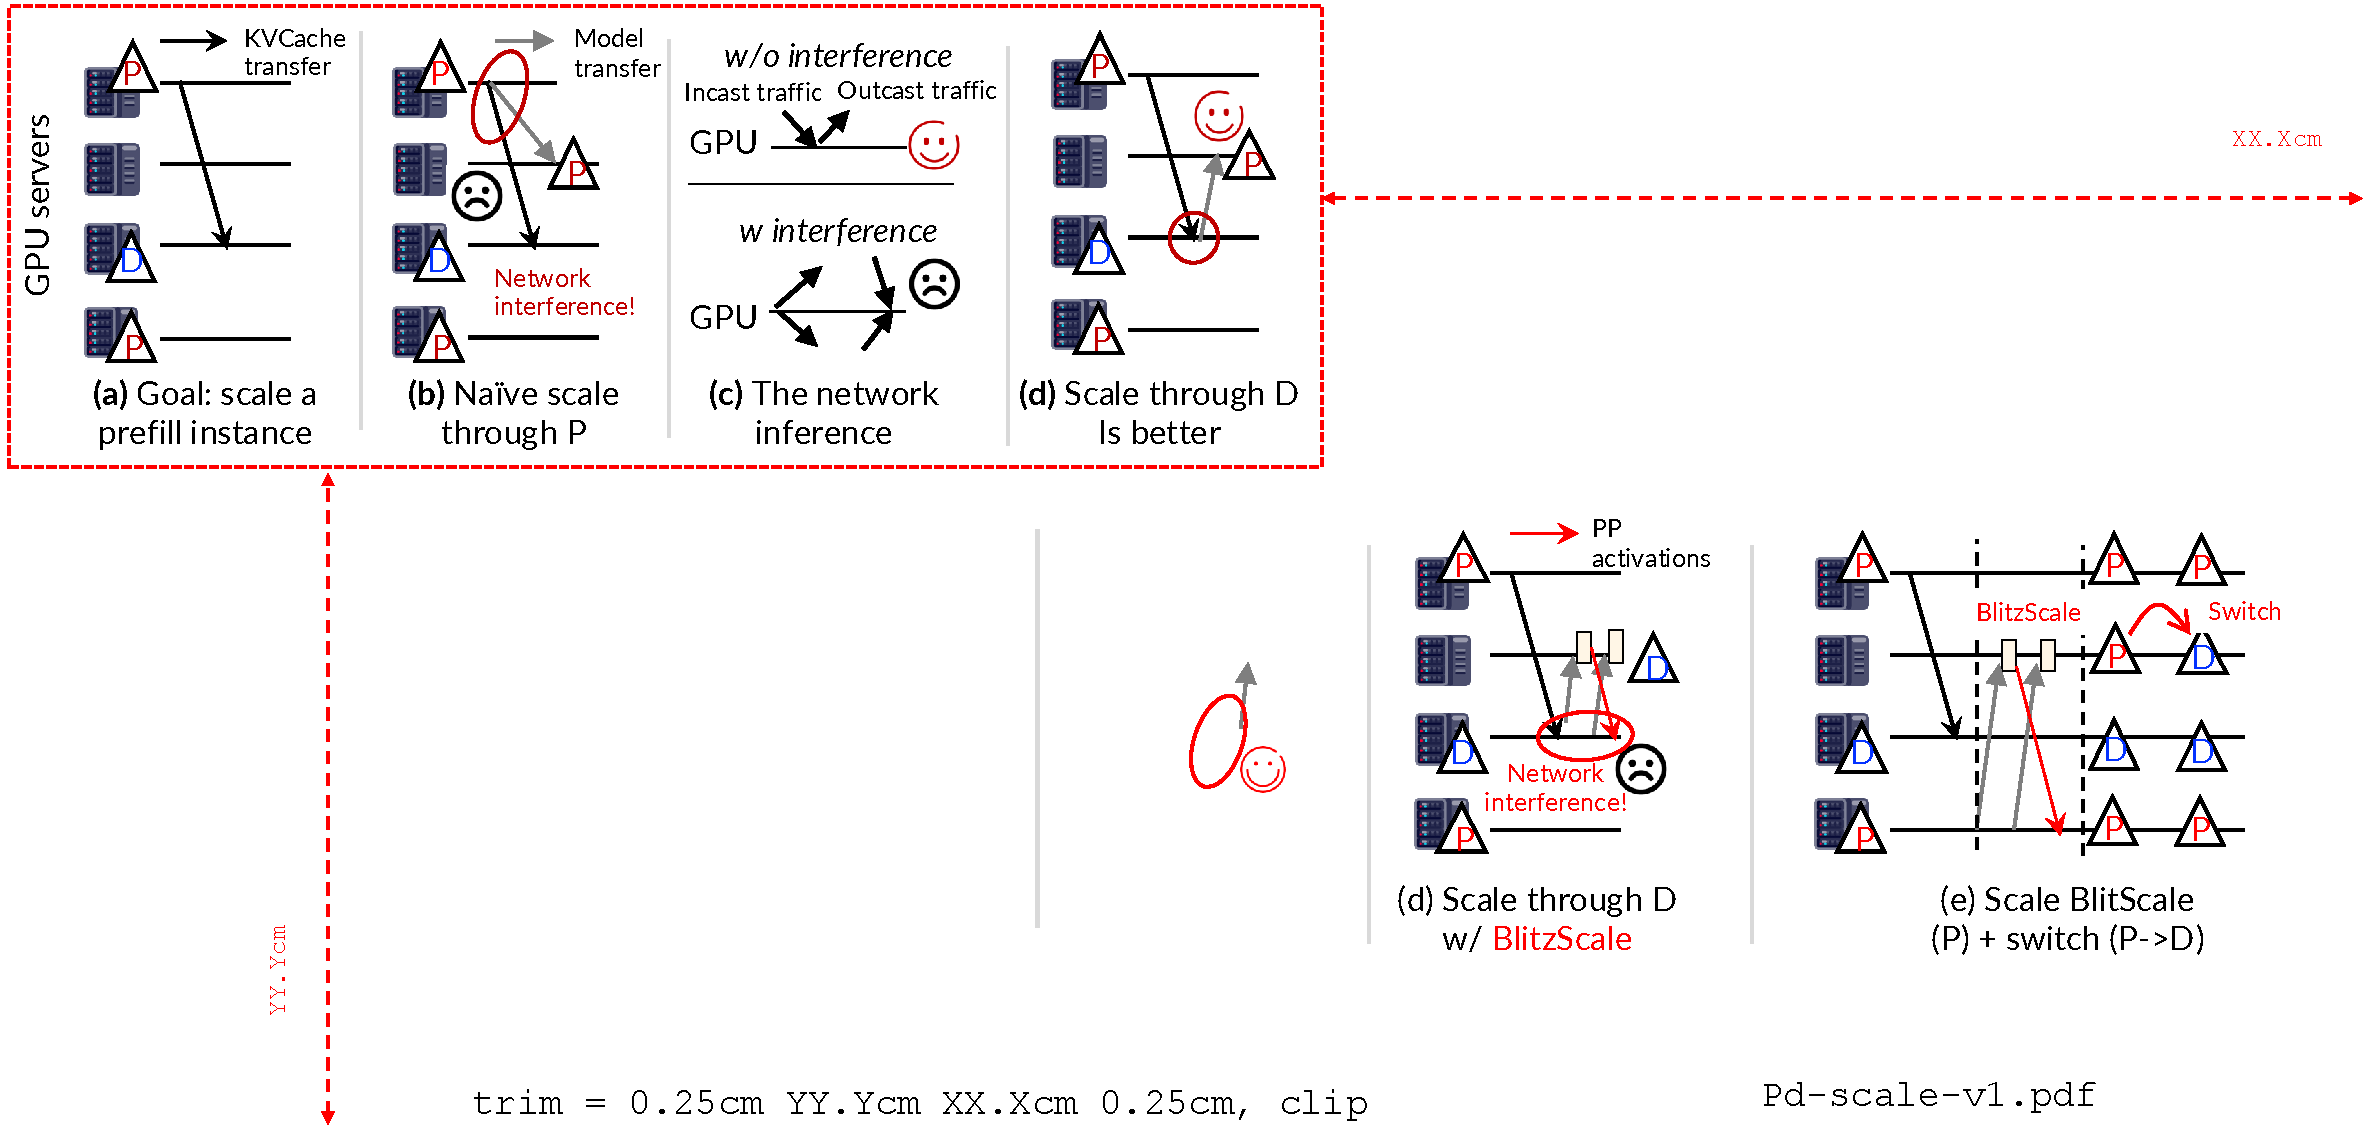
\includegraphics[width=.99\columnwidth, trim=0.25cm 11.3cm 17.7cm 0.25cm, clip]{figs/pd-scale-v1.pdf} \\[1pt]
    \end{minipage} \\[5pt]
    \begin{minipage}{1\linewidth}
        \caption{\small{\textit{
            (a) 在 LLM 的 Prefill/Decode 解耦服务中，扩一个 prefill 实例的示意图；
            (b) 如果直接从 prefill 实例扩缩，会引入网络干扰；
            (c) 利用现代数据中心网络的双向特性可以避免这种干扰；
            (d) 在考虑双向特性后得到的更优扩缩计划。
        }}}
        \label{fig:pd-scale}
    \end{minipage} \\[-10pt]
\end{figure}

\begin{figure}[!t]
    \centering
    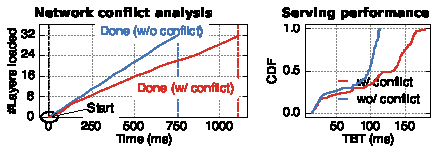
\includegraphics[left, scale=1.1]{./data/motiv-netconflict.pdf} \\[0pt]
    \begin{minipage}{1\linewidth}
        \caption{\small{\textit{
            网络干扰对 (a) 扩缩速度与 (b) 服务性能的影响分析。
        }}}
        \label{fig:motiv-network-conflict}
    \end{minipage} \\[-5pt]
\end{figure}

\stitle{挑战与方法。\,}
尽管我们利用了高速网络，
要让自动扩缩容同时具备“快速”和“在线”两种能力，
仍需解决以下挑战。

\emph{\textbf{挑战 1：在线生成无干扰的扩缩计划。} }
生成扩缩计划与生成\emph{多播}计划~\cite{DBLP:journals/jpdc/BhatRP03,DBLP:conf/asplos/CowanMMSX23,DBLP:conf/sc/GhazimirsaeedZR20,DBLP:conf/icpp/BanikazemiMP98,DBLP:conf/dsn/BehrensJBT18} 十分相似，
即如何把数据（这里是参数）从若干源快速分发到目标节点。
但自动扩缩容还有两项额外要求。
第一，计划必须能够在线生成，
因为源与目标会动态变化，
而在异构网络上求最优计划是 NP-hard 的~\cite{DBLP:journals/jpdc/BhatRP03}。
第二，计划必须消除参数加载与在线服务之间的网络干扰。
{\fig{fig:pd-scale}} 给出了采用 PD 解耦时的一个例子。
在这种设置下，
KVCache 会从 prefill 实例迁移到 decode 实例（见 (a)），
且这一迁移开销在正常情况下是可以被隐藏的~\cite{DBLP:conf/isca/PatelCZSGMB24}。
然而，如果我们想扩一个新的 prefill 实例，
并且像 (b) 那样直接把某个 prefill 实例选为参数源，
那么扩缩流量就会与 KVCache 迁移流量争夺网络带宽，
最终导致扩缩时间延长 1.5\,$\times$，
并使尾部 TBT 因 KVCache 迁移开销被放大而上升 50\,\%
（见 {\fig{fig:motiv-network-conflict}} (b)）。

针对这一问题，
我们基于三个观察设计了一个由服务负载指导的贪心计划生成方法（见 \textsection{\ref{sec:design-plan}}）。
第一，网络异构性的主要来源是 NVLink，
而 NVLink 的速度极高：
例如它能在 120\,ms 内把一个 Llama3-8B 广播到 8 张 GPU 上。
因此，我们可以把通过 NVLink 相连的实例抽象成一个逻辑实例组，
从而在规划时把 NVLink 从网络拓扑中消去。
第二，通过网络加载参数是一个带宽密集型过程，
因此我们可以用串行转发链~\cite{DBLP:conf/icpp/VerstoepLB96} 的方式贪心构造多播，
这在常见场景下是最优的。
第三，GPU 服务器之间的 RDMA 网络通常具备双向特性~\cite{288657,rdma-bidirectional}，
也就是说，入向（incast）与出向（outcast）流量不会相互干扰（见 (c)）。
因此，我们可以在计划生成时移除那些会在同一链路、同一方向上产生冲突的流，
从而规避干扰。
例如，我们可以像 {\fig{fig:pd-scale}} (d) 那样，
从 decode 实例向 prefill 实例加载参数。

\begin{figure*}[!t]
    \begin{minipage}{1\linewidth}
        \hspace{-1mm}
        \centering
        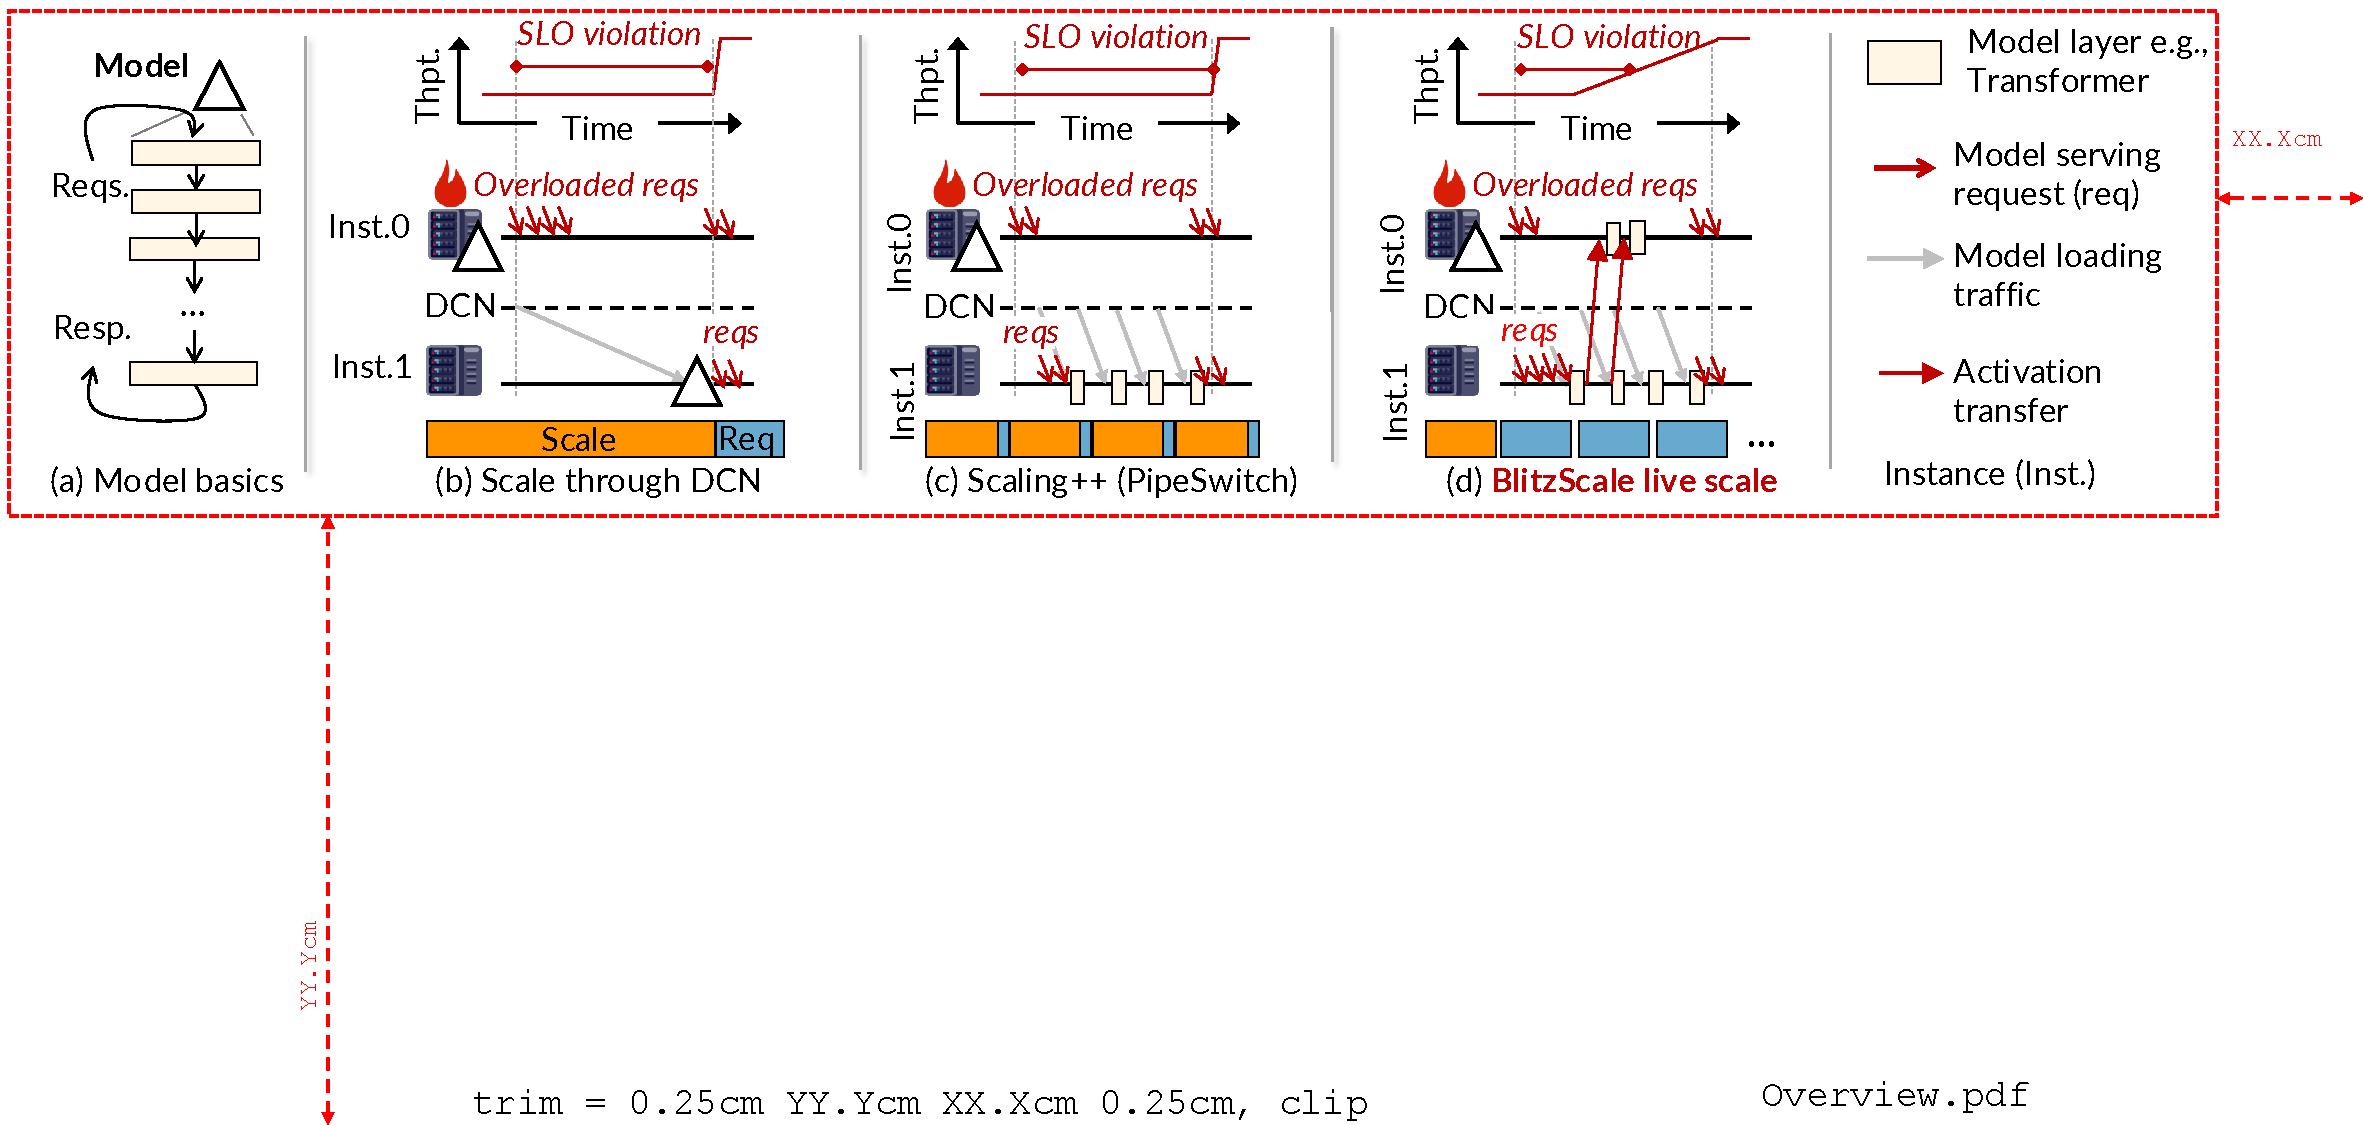
\includegraphics[width=.95\columnwidth, trim=0.25cm 10.38cm 2.5cm 0.25cm, clip]{figs/overview.pdf}
    \end{minipage} \\[8pt]
    \begin{minipage}{1\linewidth}
        \caption{\small{\textit{
            (a) 模型执行请求的整体过程；
            (b) 通过数据中心网络（DCN）进行朴素模型扩缩的示意；
            (c) 一种与执行重叠的改进扩缩方式~\cite{pipeswitch}，但它仍然不是在线的；
            (d) {\sys} 如何实现在线扩缩。
        }}}
        \label{fig:overview}
    \end{minipage} \\[-10pt]
\end{figure*}

\vspace{1.ex}
\emph{\textbf{挑战 2：实现在线自动扩缩容。} }
在线自动扩缩容——即在所有参数尚未加载完成之前，新实例就能提升系统吞吐——之所以必要，
是因为即便使用了高速网络，
仍然可能出现 SLO 违约（见 {\fig{fig:motiv-scale-speed}} (c)）。
而现有系统很难做到这一点。
例如，PipeSwitch~\cite{pipeswitch} 与 DeepPlan~\cite{deepplan}
都利用模型逐层执行的特性来进行推理。
如 {\fig{fig:overview}} (c) 所示，
一旦 inst.1 上的第一层加载完成，
它们就会把过载请求重定向给 inst.1 执行；
同时，inst.1 会并行加载后续层。
但这样的重叠并不是真正的在线扩缩，
因为在所有层都加载完成之前，
inst.1 依然无法独立完成一个请求，
也就无法真正提升系统整体吞吐。

为此，
我们提出了一种新的协同执行方案来实现在线自动扩缩容。
核心观察在于：
虽然新扩出的实例在所有层加载完之前无法独立完成请求，
但它可以利用已经加载好的层去分担过载实例上的部分计算，
从而提升整体服务吞吐。
{\fig{fig:overview}} (d) 展示了这一思想。
当 inst.0 过载、而 inst.1 正在扩缩时，
在 inst.1 加载完第一层之后，
我们会把所有请求从 inst.0 重定向到 inst.1 执行第一层。
当 inst.1 完成第一层计算后，
它再把 activation 发回 inst.0，
由 inst.0 执行剩余层。
这样一来，
系统吞吐会上升，排队时延随之下降。
要理解吞吐为何增加，
可以考虑一个 7 层模型：
若只有 inst.0 单独服务，其吞吐为 1/7；
在我们的在线扩缩方式下，
一旦 inst.1 加载好 1 层，inst.0 只需执行剩下 6 层，
其等效吞吐就提升到 1/6。
随着 inst.1 加载的层数继续增加，
吞吐还会进一步提高；
当一半层加载完成时——也就是扩缩时间过去一半时——系统吞吐达到峰值（翻倍）。
\textsection{\ref{sec:design-pp}} 将进一步介绍我们用于协调过载实例与新实例的 ZigZag 调度方法，
以在在线扩缩过程中获得最佳性能。
